\documentclass[english, 11pt]{article}
\usepackage{notes}
\usepackage{lipsum}

%Global Course Variables
\newcommand{\myCourseCode}{EECS 445}
\newcommand{\myCourseName}{Introduction to Machine Learning}
\newcommand{\myProf}{Honglak Lee}
\newcommand{\myTerm}{Fall 2015}

%Headers
\lhead{\myCourseName}
\rhead{\fancyplain{}{\rightmark}} 

%Footers
\cfoot{\thepage}

\begin{document}
\titleHeader{\myCourseCode}{\myCourseName}{\myProf}{\myTerm}

%Document information
\rule[0.5ex]{1\columnwidth}{.5pt}
Contributors: Max Smith
\begin{center}
	Latest revision: \today
\end{center}
\toc
\abstr{Theory and implementation of state-of-the-art machine learning algorithms for large-scale real-world applications. Topics include supervised learning (regression, classification, kernel methods, neural networks, and regularization) and unsupervised learning (clustering, density estimation, and dimensionality reduction).}

%----------------------------
%Document Begins
%----------------------------
% Unnamed Examples:

\begin{defn}
	A relative path is a path that is referring to your current directory.
\end{defn}

\begin{rem}
	Recall that double quotes do not protect back quotes.
\end{rem}

\begin{exmp}
	$$2+2=3$$
\end{exmp}

With some names:
\begin{defn}[Relative Path]
    A relative path is a path that is referring to your current directory.
\end{defn}

\begin{rem}[Double Quotes]
    Recall that double quotes do not protect back quotes.
\end{rem}

\begin{exmp}[Addition]
    $$2+2=3$$
\end{exmp}

\section{Readings}
\subsection{Probability Distributions}
\begin{defn}[Binary Variable]
	Single variable that can take on either 1, or 0; $x\in \{0, 1\}$. We denote $\mu$ ($0\leq\mu\leq 1$) to be the probability that the random binary variable $x=1$
	$$p(x=1|\mu)=\mu$$
	$$p(x=0|\mu)=1-\mu$$
\end{defn}

\begin{defn}[Bernoulli Distribution]
	Probability distribution of the binary variable x, where $\mu$ is the probability $x=1$.
	$$\text{Bern}(x|\mu)=\mu^x(1-\mu)^{1-x}$$
	The distribution has the following properties:
	\begin{itemize}
		\item $\text{E}(x)=\mu$
		\item $\text{Var}(x)=\mu (1-\mu)$
		\item $\mathcal{D}=\{x_1,\ldots ,x_N\} \to p(\mathcal{D} | \mu )=\Pi_{n=1}^{N}p(x_n|\mu)$
		\item Maximum likelihood estimator: $\mu_{ML}=\frac{1}{N}\sum_{n=1}^{N}x_n=\frac{numOfOnes}{sampleSize}$ (aka. sample mean)
	\end{itemize}
\end{defn}

\begin{defn}[Binomial Distribution]
	Distribution of $m$ observations of $x=1$, given a sample size of $N$. 
	$$\text{Bin} (m|N,\mu={\substack{N\\m}}\mu^m (1-\mu )^{N-m}$$\
	\begin{itemize}
		\item $\text{E}(m)=N\mu$
		\item $\text{Var}(m)=N\mu (1-\mu )$
	\end{itemize}
\end{defn}

\subsubsection{The Beta Distribution}
In order to develop a Bayesian treatment for fitting data sets, we will introduce a prior distribution $p(\mu)$.

\begin{itemize}[--]
	\item \textbf{Conjugacy:} when the prior and posterior distributions belong to the same family.
\end{itemize}

\begin{defn}[Beta Distribution]
	$$\text{Beta}(\mu |a,b)=\frac{\Gamma (a+b)}{\Gamma (a)\Gamma (b)}\mu^{a-1} (1-\mu )^{b-1}$$
	Where $\Gamma (x)$ is the gamma function.
	The distribution has the following properties:
	\begin{itemize}
		\item $\text{E}(\mu )=\frac{a}{a+b}$
		\item $\text{Var}(\mu )=\frac{ab}{(a+b)^2 (a+b+1)}$
		\item conjugacy
		\item ${a\to\infty || b\to\infty}\to \text{variance}\\to 0$ 
	\end{itemize}

	Conjugacy can be shown by the distribution by the likelihood function (binomial):
	$$p(\mu |m,l,a,b)\propto \mu^{m+a-1} (1-\mu )^{l+b-1}$$
	Normalized to:
	$$p(\mu |m,l,a,b)= \frac{\Gamma (m+a+l+b)}{\Gamma (m+a)\Gamma (l+b)} \mu^{m+a-1} (1-\mu )^{l+b-1}$$
\end{defn}

\begin{itemize}[--]
	\item \textbf{Hyperparameters:} parameters that control the distribution of the regular parameters.
	\item \textbf{Sequential Approach:} method of learning where you make use of an observation one at a time, or in small batches, and then discard them before the next observatiosn are used. (Can be shown with a Beta, where observing $x=1\to a++, x=0\to b++$, then normalizing)
	\item For a finite data set, the posterior mean for $\mu$ always lies between the prior mean and the maximum likelihood estimate.
	\item A general property of Bayesian learning is when we observe more and more data the uncertainty of the posterior distribution will steadily decrease.
	\item More information and examples of probability distributions can be found in Appendix B of Bishop's `Pattern Recognition and Machine Learning.'
\end{itemize}


\subsection{Linear Models for Regression}
\begin{itemize}[--]
	\item \textbf{Linear Regression:} $y(\mathbf{x}, \mathbf{w})=w_0+w_1 x_1+\ldots +w_D x_D$
	\item Limited on linear function of input variables $x_i$
	\item Extend the model with nonlinear functions, where $\phi_j (x)$ are known as basis functions:
		$$y(\mathbf{x}, \mathbf{w})=w_0 +\sum_{j=1}^{M-1}w_j\phi_j (x)$$
	\item $w_0$ allows for any fixed offset in data, and is known as the \textbf{bias parameter}.
	\item Given a dummy variable $\phi_0 (x)=1$, our model becomes:
		$$y(\mathbf{x}, \mathbf{w})=\sum_{j=0}^{M-1}w_j\phi_j (x)=\mathbf{W}^\mathbf{T} \mathbf{\phi} (x)$$
	\item Functions of this form are called \textbf{linear models} because the function is linear in weight.
\end{itemize}

\subsubsection{Maximum likelihood and least squares}
\begin{itemize}[--]
	\item j
\end{itemize}

\section{Stanford Notes}
\subsection{Linear Regression with One Variable}
\subsubsection{Model Representation}
\begin{itemize}[--]
	\item Goal is model labelled data (data which we have the correct output for) to a line 
	\item Notation:\begin{description}
		\item[$m$] = number of training examples
		\item[$x$] = input variable/feature
		\item[$y$] = output variable/feature
		\item[$(x,y)$] = one training example
		\item[$(x^{(i)},y^{(i)})$] = $i$th training example (parens indicate index)
	\end{description}

	\item We take a training set, input into a learning algorithm, which returns a hypothesis ($h$) that models the relationship.
	\begin{center}\begin{tikzpicture}[node distance = 2cm, auto]
		%Place nodes
		\node [block] (train) {Training Set};
		\node [block, below of=train] (alg) {Learning Algorithm};
		\node [block, below of=alg] (hyp) {$h$};
		\node [cloud, left of=hyp] (x) {$x$};
		\node [cloud, right of=hyp] (y) {$y$};

		%Draw edges
		\path [line] (train) -- (alg);
		\path [line] (alg) -- (hyp);
		\path [line] (x) -- (hyp);
		\path [line] (hyp) -- (y);
	\end{tikzpicture}\end{center}
	\item $h$ maps from $x$'s to $y$'s ($h(x)=y$).
	\item We need to determine how we want to represent $h$
	\item A simple linear model with one variable for $h$ is: $$h_\theta (x) = \theta_0 + \theta_1 x$$, called \textbf{univariate linear regression}.
\end{itemize}

\subsubsection{Cost Function}
\begin{itemize}[--]
	\item Given a hypothesis: $h_\theta (x) = \theta_0 + \theta_1 x$
	\begin{description}
		\item[$\theta_i's$] = parameters of the model
	\end{description}

	\item We will now discuss how to choose the parameters of our model
	\item Idea: choose $\theta_0, \theta_1$ so that $h_\theta (x)$ is close to $y$ for our training examples $(x,y)$
	\item We want to minimize $\theta_0, \theta_1$ such that $h(x) - y$ is minimal (reminder: $h(x)$ is the guess at the correct value at $y$).
	\item Because we we only are looking to minimize our absolute distance, we square the distance we want to minimize to account for positive and negative differences equally now making our cost function: $(h(x)-y)^2$
	\item However, we don't want to minimize it for just one example, so we do this for every training example: $$\sum_{i=1}^{m}(h_\theta (x^{(i)}) - y^{(i)})^2$$
	\item To make later math easier, we further refine our formula to be half the average: $$\frac{1}{2m}\sum_{i=1}^{m}(h_\theta (x^{(i)}) - y^{(i)})^2$$
	\item This function we created is called our \textbf{cost} function, as it measures how expensively incorrect our current model is, which we will denote with $J$. 
	\item The cost function is dependent on the hypothesis parameters, and our goal is to adjust these parameters to minimize the overrall cost of our model: $$J(\theta_0, \theta_1) = \frac{1}{2m}\sum_{i=1}^{m}(h_\theta (x^{(i)}) - y^{(i)})^2$$
	\item Now our goal is to minimize $J$ over the variables $\theta_0, \theta_1$
\end{itemize}

\subsubsection{Cost Function - Intuition I}
\begin{center}
	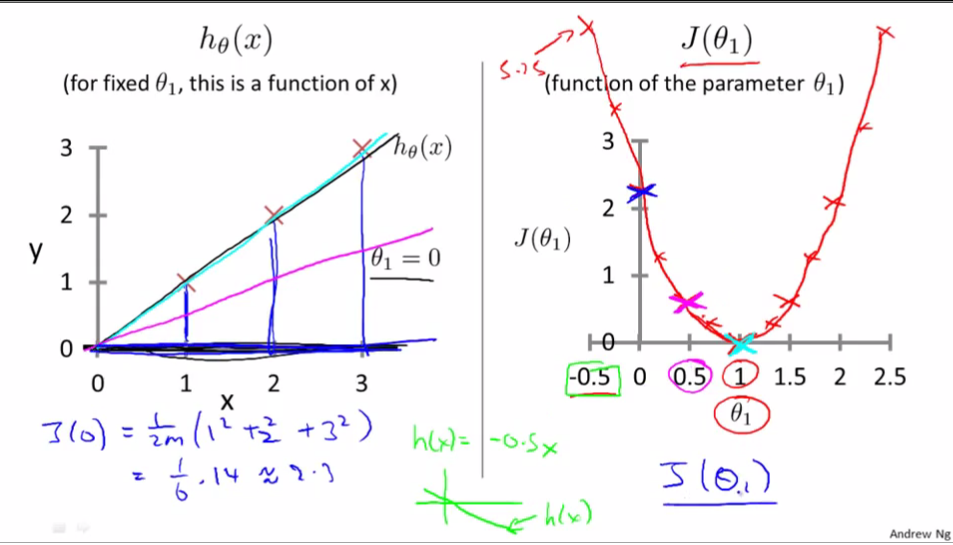
\includegraphics[scale=0.75]{sections/cs229/w1/cost_function.png}
\end{center}
This image shows that for varying parameter values, the cost function changes. In this idealistic example there's a global minimum, the goal of minimized cost, that is very easily followed by a hill-climbing style algorithm.

\subsubsection{Cost Function - Intuition II}
\begin{center}
	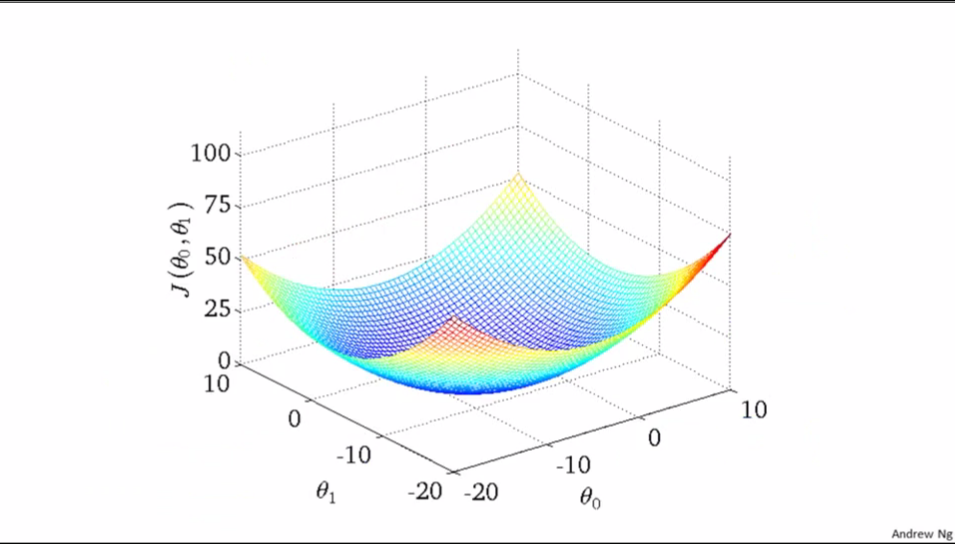
\includegraphics[scale=0.75]{sections/cs229/w1/2d_cost_function.png}
\end{center}
Similarly when you have an additional variable, you want to reach the bottom of this $N$-dimensional hill (note: not all models will have such a perfect hill). 
\begin{itemize}[--]
	\item The gradient gives the direction of maximumal increase on a surface.
	\item We will use a negative gradient to find the `direction' to travel towards the bottom of the hill
	\item Another common way to represent multidimensional cost functions is through contour plots
	\item 
\end{itemize}

% \section{Introduction and Overview}
% \section{Supervised Learning: Regression}
% \section{Supervised Learning: Classification}
% \section{Kernel Methods}
% \section{Regularization and Model Selection}
% \section{Advice on using ML Algorithms}
% \section{Neural Networks}
% \section{Unsupervised Learning}
% \section{Gaussian Process}
% \section{Ensemble Methods}
% \section{Sequence Modeling}
% \section{Learning Theory}

\end{document}